\documentclass[preprint,review,12pt]{elsarticle}
% template: elsevier — elsarticle.cls comes from https://ctan.org/pkg/elsarticle and is not shipped with the fixture
\usepackage{graphicx}
\usepackage{amsmath,amssymb}
\usepackage{booktabs}
\usepackage{subcaption}
\usepackage{algorithm}
\usepackage{algpseudocode}
\graphicspath{{../../figures/}}

\begin{document}
\begin{frontmatter}
\title{Domain-robust vision-based force estimation by removing the platform sensor offset}
\author[1]{Anonymous}
\affiliation[1]{organization={Fixture University}, city={Nowhere}, country={Nowhere}}
\begin{abstract}
Vision-based force estimation degrades across robot platforms because of a label-side sensor offset. A domain-adversarial regularizer removes it and lowers the root-mean-square error (RMSE) on the held-out platform by 19.2\% relative to the strongest baseline.
\end{abstract}
\begin{keyword}
force estimation \sep domain shift \sep surgical robotics
\end{keyword}
\end{frontmatter}

\section{Introduction}
Surgical force estimation must transfer across robot platforms~\cite{lecun2015deep}. Fig.~\ref{fig:main} summarises the main comparison, Fig.~\ref{fig:abl} the ablations, and Table~\ref{tab:main} the numbers. The strongest baseline is the geometric regressor of~\cite{he2016resnet}.

\section{Method}
The objective is $L = L_{reg} + \beta L_{dom} + \alpha L_{cons}$. Algorithm~\ref{alg:train} summarises the training procedure.

\begin{algorithm}[t]
\caption{Training with the domain-adversarial and the consistency term.}
\label{alg:train}
\begin{algorithmic}[1]
\Require encoder with heads $f_\theta$, training loader $\mathcal{D}$, $\beta = 0.1$, $\alpha = 0.5$, $K = 3$
\Ensure trained parameters $\theta$ and the loss history $h$
\State $h \gets \emptyset$
\For{$k = 1, \ldots, K$}
  \State $L \gets L_{reg}(f_\theta, \mathcal{D})$
  \If{$\beta > 0$}
    \State $L \gets L + \beta\, L_{dom}$
  \EndIf
  \If{$\alpha > 0$}
    \State $L \gets L + \alpha\, L_{cons}$
  \EndIf
  \State $h \gets h \cup \{\textsc{Step}(L)\}$
\EndFor
\State \Return $h$
\end{algorithmic}
\end{algorithm}


\begin{figure}[t]
  \centering
  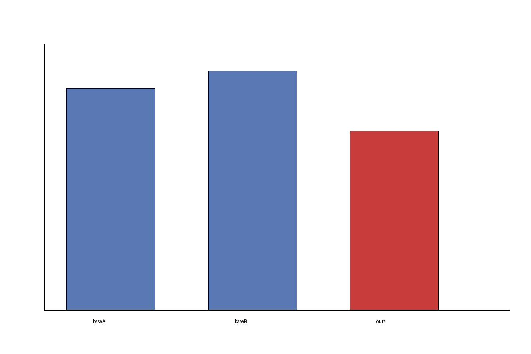
\includegraphics[width=0.47\textwidth]{fig_main.pdf}
  \caption{Main comparison on both platforms (fixture).}
  \label{fig:main}
\end{figure}

\begin{figure}[t]
  \centering
  \begin{subfigure}[t]{0.48\textwidth}
    \centering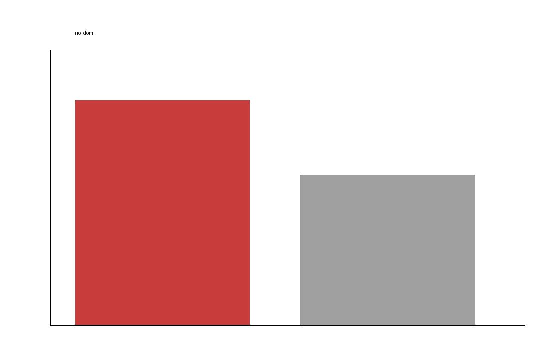
\includegraphics[width=\linewidth]{fig_abl_a.pdf}
    \caption{Removing the adversarial term.}\label{fig:abl-a}
  \end{subfigure}\hfill
  \begin{subfigure}[t]{0.48\textwidth}
    \centering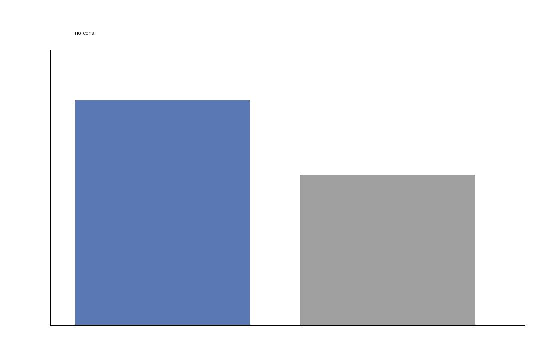
\includegraphics[width=\linewidth]{fig_abl_b.pdf}
    \caption{Removing the consistency term.}\label{fig:abl-b}
  \end{subfigure}
  \caption{Ablations composed in LaTeX from one PDF per panel.}
  \label{fig:abl}
\end{figure}


\section{Experiments}
\begin{table}[t]
  \centering
  \caption{Main comparison, contact-window convention.}
  \label{tab:main}
  \begin{tabular}{lcc}
    \toprule
    Method & RMSE E1 (N) & RMSE E2 (N) \\
    \midrule
    baseA & 0.250 & 0.352 \\
    ours & 0.202 & 0.303 \\
    \bottomrule
  \end{tabular}
\end{table}

\section{Conclusion}
The gain comes from the adversarial term.

\bibliographystyle{elsarticle-num}
\bibliography{../refs}
\end{document}
